\documentclass[a4paper]{scrbook}

\usepackage{fullpage}
\usepackage{style}

\newif\iffigureon
\figureonfalse


% THEOREM ENVIORMMENT e.g. \newtheorem{comando}{nome}[numerazione]
\theoremstyle{definition}
\newtheorem{definition}{Definizione}[chapter]
\newtheorem{example}{Esempio}[chapter]
\newtheorem{exercise}{Esercizio}[chapter]

\numberwithin{equation}{chapter}

\title{Introduzione ai sistemi dinamici I}
\author{SciSNS-2017}

\begin{document}
	
\frontmatter

\maketitle

Quest'opera è stata rilasciata con licenza Creative Commons Attribuzione - Condividi allo stesso modo 4.0 Internazionale. Per leggere una copia della licenza visita il sito web Quest'opera è stata rilasciata con licenza Creative Commons Attribuzione - Non commerciale - Condividi allo stesso modo 4.0 Internazionale. Per leggere una copia della licenza visita il sito web \url{http://creativecommons.org/licenses/by-nc-sa/4.0/}.
\iffigureon
\begin{center}
	\href{http://creativecommons.org/licenses/by-nc-sa/4.0/}{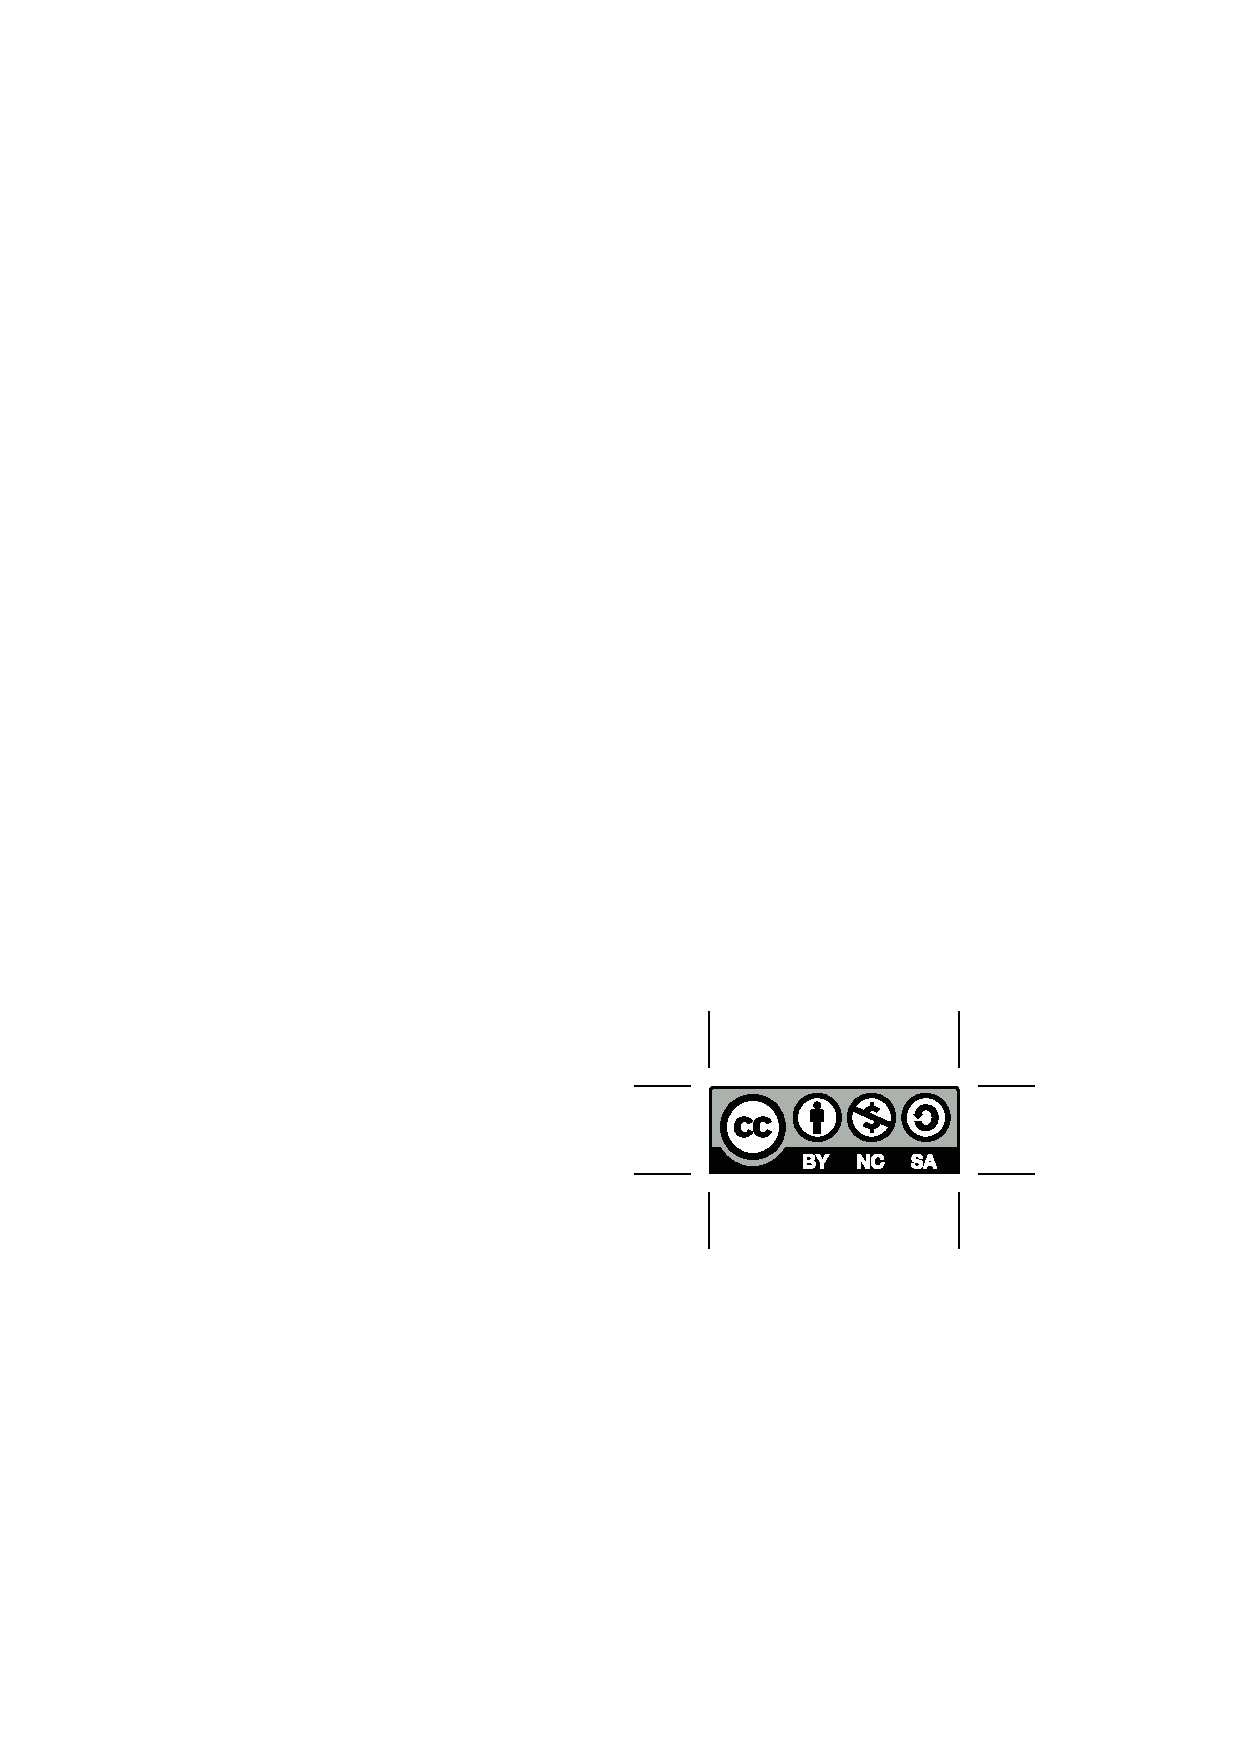
\includegraphics[scale = 0.8]{img/by-nc-sa}}
\end{center}
\fi	


\tableofcontents


\mainmatter

\chapter{Lezioni}
\section{Lezione del 09/10/2018}
\begin{definition}[gruppo]
	Un gruppo è una coppia $ \mathcal{G} \coloneqq (G, \star) $ dove $ G $ è un insieme e $ + \colon G \times G \to G $ è un'operazione binaria che gode delle seguenti proprietà
	\begin{enumerate}[label=(\roman*)]
		\item \emph{associativa}: $ \forall g_1, g_2, g_3 \in G, \ g_1 \star (g_2 \star g_3) = (g_1 \star g_2) \star g_3 $;
		\item \emph{elemento neutro sinistro}: $  \exists e \in G : \forall g \in G, \ g \star e = g $;
		\item \emph{inverso sinistro}: $ \forall g \in G, \exists g^{-1} \in G : g \star g^{-1} = e $.
	\end{enumerate}
	A partire da queste si mostra facilmente che l'elemento neutro destro è anche elemento neutro sinistro, l'inverso destro è anche inverso sinistro, che l'elemento neutro e l'inverso sono unici. \\
	Se non ci sono ambiguità circa l'operazione definita su $ G $ indicheremo più semplicemente il gruppo $ \mathcal{G} $ facendo riferimento al solo insieme $ G $. 
\end{definition}

\begin{definition}[sistema dinamico]
	Un sistema dinamico è una terna $ (\mathcal{G}, \mathcal{X}, \Phi) $ dove $ \mathcal{G} \coloneqq (G, \star) $ è un (semi-)gruppo, $ \mathcal{X} $ è uno spazio, cioè un insieme $ X $ dotato di una qualche struttura (per esempio una topologia), e 
	\begin{align*}
		\Phi \colon G \times X & \to X \\
		(g, x) & \mapsto \Phi(g, x) = \Phi_g(x)
	\end{align*}
	è una applicazione tale che
	\begin{enumerate}[label=(\roman*)]
		\item $ \forall x \in X, \ \Phi_e(x) = x $ dove $ e $ è l'elemento neutro di $ G $, cioè $ \Phi_e = \Id_X $;
		\item $ \forall g_1, g_2 \in G, \forall x \in X, \ \Phi_{(g_1 \star g_2)}(x) = (\Phi_{g1} \circ \Phi_{g_2})(x) $ cioè $ \Phi_{(g_1 \star g_2)} = \Phi_{g1} \circ \Phi_{g_2} $.
	\end{enumerate}
	Più brevemente diciamo che un sistema dinamico è l'\emph{azione} di un gruppo $ G $ su uno spazio $ X $ definita da una mappa $ \Phi $. 
\end{definition}

Nella maggior parte dei casi useremo come gruppo insiemi numerici $ \N $, $ \Z $ e $ \R $ con le usuali operazioni. Nei primi due casi parleremo di sistemi a \emph{tempo discreto} mentre nell'ultimo di sistemi a \emph{tempo continuo}. Come spazio $ \mathcal{X} $ useremo spesso uno \emph{spazio metrico compatto} (e.g. la sfera $ \S^d $, il toro $ \T^d $ o un intervallo chiuso $ [a, b] $), uno \emph{spazio di probabilità} o gli insiemi $ \R^d $ e $ \C $ con le usuali strutture. \\

Per quanto riguarda la mappa $ \Phi $ osserviamo che per definizione $ \Phi_g \in \End{(X)} $ ovvero è un \emph{endomorfismo} su $ X $. Tuttavia spesso penseremo a $ \Phi_g \in \Aut{(X)} $ ovvero un \emph{automorfismo} cioè un endomorfismo invertibile. \\

Sia $ f \in \End{(X)} $. Dato $ n \in \N $ poniamo $ f^n \coloneqq f \circ \cdots \circ f $ ($ f $ composta $ n $ volte) con la convenzione che $ f^1 = f $ e $ f^0 = \Id_X $. Se consideriamo $ \N $ con l'operazione di addizione, l'applicazione $ \Phi^f $ data da $ \Phi_n^f(x) \coloneqq f^n(x) $ definisce un sistema dinamico. \\
Se prendiamo $ f \in \Aut{(X)} $ possiamo considerare la stessa costruzione usando come gruppo $ \Z $ e definendo $ f^{-n} $ come l'inversa di $ f^n $. 

\begin{example}
	Partendo dalla costruzione appena data possiamo prendere $ X = [0, 1] $ e per $ \alpha \in \R $ la funzione $ f(x) \coloneqq x + \alpha \pmod{1} $. Osserviamo che essendo $ f $ invertibile possiamo definire l'applicazione $ \Phi $ su $ \Z $. Il sistema così definito è un prototipo di \emph{sistema periodico} se $ \alpha \in \Q $ e di \emph{sistema quasi-periodico} se $ \alpha \notin \Q $. \\
	\texttt{Sarebbe carino mettere un'immagine.}
\end{example}

Prendiamo come gruppo $ \R $ o $ [0, +\infty) $. In tale caso data l'applicazione $ \Phi_t(x) = \Phi(t, x) $ prende il nome di \emph{flusso} o \emph{semi-flusso} rispettivamente. \\

Un esempio di sistema dinamico a tempo continuo è dato da un'equazione differenziale ordinaria (ODE) del primo ordine \footnote{Di seguito considereremo quasi solo ODE del primo ordine in quanto equazioni differenziali di ordine superiore possono essere ricondotte a questa con il solito cambio di variabile a sistemi di ODE del primo ordine.} autonoma
\begin{equation}
	\begin{cases}
		\dot{x} = v(x) \\
		x(0) = x_0
	\end{cases}
\end{equation} 
dove $ x, x_0 \in \R^n $ e $ v \colon \R^n \to \R^n $ è un campo vettoriale. Se supponiamo che $ v $ sia di classe $ \mathcal{C}^1 $ allora abbiamo esistenza e unicità della soluzione \texttt{(e dipendenza continua dai parametri iniziali ??)}, cioè esiste $ \tau > 0 $ e un'unica funzione $ \phi \colon [0, \tau) \to \R^n $ tale che $ \phi(0) = x_0 $ e $ \phi'(t) = v(\phi(0)) $ per ogni $ t \in [0, \tau) $. \\
Se supponiamo per esempio che $ v $ sia un'applicazione lineare $ v(x) \coloneqq A x $ con $ A \in \mathrm{Mat}_{n \times n}(\R) $ allora abbiamo che la soluzione è prolungabile a tutto l'asse reale e introducendo la nozione di esponenziale di una matrice %
\footnote{%
	Data $ A \in \mathrm{Mat}_{n \times n}(\R) $ si pone 
	\[
		\exp(A) \coloneqq \sum_{k = 0}^{+\infty} \frac{A^k}{k!}.
	\] 
} si può scrivere nella forma 
\[
	\phi(t) = \exp{\left(t \, A\right)} \, x_0. 
\]


\begin{definition}[orbita e spazio delle orbite]
	Data $ f \in \Aut{(X)} $ e $ \Phi^f \colon \Z \times X \to X $ definiamo orbita di $ x \in X $ come 
	\[
	\mathcal{O}^f(x) \coloneqq \{f^n(x) : n \in \Z\}.
	\]
	Le orbite definiscono una naturale relazione di equivalenza $ x \sim y \iff \exists n \in \Z : y = f^n(x) \iff y \in \mathcal{O}^f(x) \iff x \in \mathcal{O}^f(y) $. Chiamiamo lo spazio quoziente $ \faktor{X}{\sim} $ spazio delle orbite. \texttt{Topologia quoziente?}
\end{definition}

Pendolo semplice...

\section{Lezione del 10/10/2018}
\subsection{Introduzione}
La Teoria della Misura nasce a inizio '900 per formalizzare la probabilità e per cercare di fondare una teoria dell'integrazione che risulti più efficace di quella di Riemann. Per alcuni sottoinsiemi di $\R$, in particolare per gli intervalli limitati, abbiamo un concetto intuitivo di "misura", ovvero la lunghezza dell'intervallo:
\[\lambda\left([a,b]\right) = b-a.\]
L'obiettivo della teoria della misura è estendere questa nozione ad altri sottoinsiemi di $\R$ in modo coerente, ovvero in modo da rispettare, ad esempio, la proprietà di additività:
\[A \cap B = \emptyset \implies \lambda(A\cup B) = \lambda(A) + \lambda(B)\]


\appendix

\chapter{Appendice}


\backmatter

%\bibliography{bibliografia}


\end{document}